\documentclass[12pt,twoside]{article}
%%%%%%%%%%%%%%%%%%%%%%%%%%%%%%%%%%%%%%%%%%%%%%%%%%%%%%%%%%%%%
% Meta informations:
\newcommand{\trauthor}{Michael Blesel, Oliver Pola}
\newcommand{\trtype}{Seminar Paper} %{Seminararbeit} %{Proseminararbeit}
\newcommand{\trcourse}{Neural Networks}
\newcommand{\trtitle}{Boltzmann Machine}
\newcommand{\trmatrikelnummer}{6443269, 6769946}
\newcommand{\tremail}{\{3blesel, 5pola\}@informatik.uni-hamburg.de}
\newcommand{\trarbeitsbereich}{Knowledge Technology, WTM}
\newcommand{\trdate}{\today}

%%%%%%%%%%%%%%%%%%%%%%%%%%%%%%%%%%%%%%%%%%%%%%%%%%%%%%%%%%%%%
% Languages:

% Falls die Ausarbeitung in Deutsch erfolgt:
% \usepackage[german]{babel}
% \usepackage[T1]{fontenc}
% \usepackage[latin1]{inputenc}
% \usepackage[latin9]{inputenc}	 				
% \selectlanguage{german}

% If the thesis is written in English:
\usepackage[english]{babel} 						
\selectlanguage{english}

%%%%%%%%%%%%%%%%%%%%%%%%%%%%%%%%%%%%%%%%%%%%%%%%%%%%%%%%%%%%%
% Bind packages:
\usepackage{acronym}                    % Acronyms
\usepackage{algorithmic}								% Algorithms and Pseudocode
\usepackage{algorithm}									% Algorithms and Pseudocode
\usepackage{amsfonts}                   % AMS Math Packet (Fonts)
\usepackage{amsmath}                    % AMS Math Packet
\usepackage{amssymb}                    % Additional mathematical symbols
\usepackage{amsthm}
\usepackage{booktabs}                   % Nicer tables
%\usepackage[font=small,labelfont=bf]{caption} % Numbered captions for figures
\usepackage{xcolor}                      % Enables defining of colors via \definecolor
\definecolor{uhhRed}{RGB}{254,0,0}		  % Official Uni Hamburg Red
\definecolor{uhhGrey}{RGB}{122,122,120} % Official Uni Hamburg Grey
\usepackage{fancybox}                   % Gleichungen einrahmen
\usepackage{fancyhdr}										% Packet for nicer headers
%\usepackage{fancyheadings}             % Nicer numbering of headlines

%\usepackage[outer=3.35cm]{geometry} 	  % Type area (size, margins...) !!!Release version
%\usepackage[outer=2.5cm]{geometry} 		% Type area (size, margins...) !!!Print version
%\usepackage{geometry} 									% Type area (size, margins...) !!!Proofread version
\usepackage[outer=3.15cm]{geometry} 	  % Type area (size, margins...) !!!Draft version
\geometry{a4paper,body={5.8in,9in}}

\usepackage{graphicx}                   % Inclusion of graphics
%\usepackage{latexsym}                  % Special symbols
\usepackage{longtable}									% Allow tables over several parges
\usepackage{listings}                   % Nicer source code listings
\usepackage{lstautogobble}
\usepackage{multicol}										% Content of a table over several columns
\usepackage{multirow}										% Content of a table over several rows
\usepackage{rotating}										% Alows to rotate text and objects
\usepackage[hang]{subfigure}            % Allows to use multiple (partial) figures in a fig
%\usepackage[font=footnotesize,labelfont=rm]{subfig}	% Pictures in a floating environment
\usepackage{tabularx}										% Tables with fixed width but variable rows
\usepackage{url,xspace,boxedminipage}   % Accurate display of URLs

\usepackage{varioref}
\usepackage[hidelinks]{hyperref}
\usepackage[capitalise,noabbrev]{cleveref}
\usepackage{overpic}
\usepackage{todo}

\lstset{
	frame=single,
	aboveskip=10pt,
	belowskip=10pt,
	%basicstyle={\scriptsize\ttfamily},
	basicstyle=\footnotesize,
	numbers=left,
	numberstyle=\tiny\color{gray},
	keywordstyle=\color{magenta},
	commentstyle=\color{gray},
	stringstyle=\color{teal},
	emphstyle=\color{blue},
	language=,
	breaklines=true,
	breakatwhitespace=true,
	postbreak=\hbox{$\hookrightarrow$ },
	showstringspaces=false,
	autogobble=true,
	upquote=true,
	tabsize=4,
	captionpos=b,
	morekeywords={as,with}
}

%%%%%%%%%%%%%%%%%%%%%%%%%%%%%%%%%%%%%%%%%%%%%%%%%%%%%%%%%%%%%
% Configurationen:

\hyphenation{whe-ther} 									% Manually use: "\-" in a word: Staats\-ver\-trag

%\lstloadlanguages{C}                   % Set the default language for listings
\DeclareGraphicsExtensions{.pdf,.svg,.jpg,.png,.eps} % first try pdf, then eps, png and jpg
\graphicspath{{./src/}} 								% Path to a folder where all pictures are located
\pagestyle{fancy} 											% Use nicer header and footer

% Redefine the environments for floating objects:
\setcounter{topnumber}{3}
\setcounter{bottomnumber}{2}
\setcounter{totalnumber}{4}
\renewcommand{\topfraction}{0.9} 			  %Standard: 0.7
\renewcommand{\bottomfraction}{0.5}		  %Standard: 0.3
\renewcommand{\textfraction}{0.1}		  	%Standard: 0.2
\renewcommand{\floatpagefraction}{0.8} 	%Standard: 0.5

% Tables with a nicer padding:
\renewcommand{\arraystretch}{1.2}

%%%%%%%%%%%%%%%%%%%%%%%%%%%%
% Additional 'theorem' and 'definition' blocks:
\theoremstyle{plain}
\newtheorem{theorem}{Theorem}[section]
%\newtheorem{theorem}{Satz}[section]		% Wenn in Deutsch geschrieben wird.
\newtheorem{axiom}{Axiom}[section] 	
%\newtheorem{axiom}{Fakt}[chapter]			% Wenn in Deutsch geschrieben wird.
%Usage:%\begin{axiom}[optional description]%Main part%\end{fakt}

\theoremstyle{definition}
\newtheorem{definition}{Definition}[section]

%Additional types of axioms:
\newtheorem{lemma}[axiom]{Lemma}
\newtheorem{observation}[axiom]{Observation}

%Additional types of definitions:
\theoremstyle{remark}
%\newtheorem{remark}[definition]{Bemerkung} % Wenn in Deutsch geschrieben wird.
\newtheorem{remark}[definition]{Remark} 

%%%%%%%%%%%%%%%%%%%%%%%%%%%%
% Provides TODOs within the margin:
\newcommand{\TODO}[1]{\marginpar{\emph{\small{{\bf TODO: } #1}}}}

%%%%%%%%%%%%%%%%%%%%%%%%%%%%
% Abbreviations and mathematical symbols
\newcommand{\modd}{\text{ mod }}
\newcommand{\RS}{\mathbb{R}}
\newcommand{\NS}{\mathbb{N}}
\newcommand{\ZS}{\mathbb{Z}}
\newcommand{\dnormal}{\mathit{N}}
\newcommand{\duniform}{\mathit{U}}

\newcommand{\erdos}{Erd\H{o}s}
\newcommand{\renyi}{-R\'{e}nyi}
%%%%%%%%%%%%%%%%%%%%%%%%%%%%%%%%%%%%%%%%%%%%%%%%%%%%%%%%%%%%%
% Document:
\begin{document}
\renewcommand{\headheight}{14.5pt}

\fancyhead{}
\fancyhead[LE]{ \slshape \trauthor}
\fancyhead[LO]{}
\fancyhead[RE]{}
\fancyhead[RO]{ \slshape \trtitle}

%%%%%%%%%%%%%%%%%%%%%%%%%%%%
% Cover Header:
\begin{titlepage}
	\begin{flushleft}
		Universit\"at Hamburg\\
		Department Informatik\\
		\trarbeitsbereich\\
	\end{flushleft}
	\vspace{3.5cm}
	\begin{center}
		\huge \trtitle\\
		(DRAFT)
	\end{center}
	\vspace{3.5cm}
	\begin{center}
		\normalsize\trtype\\
		[0.2cm]
		\Large\trcourse\\
		[1.5cm]
		\Large \trauthor\\
		[0.2cm]
		\normalsize Matr.Nr. \trmatrikelnummer\\
		[0.2cm]
		\normalsize\tremail\\
		[1.5cm]
		\Large \trdate
	\end{center}
	\vfill
\end{titlepage}

	%backsite of cover sheet is empty!
\thispagestyle{empty}
\hspace{1cm}
\newpage

%%%%%%%%%%%%%%%%%%%%%%%%%%%%
% Abstract:
% Abstract gives a brief summary of the main points of a paper: \section*{Abstract}

Here will be an abstract.


% Lists:
\setcounter{tocdepth}{2} 					% depth of the table of contents (for Seminars 2 is recommented)
\tableofcontents
\pagenumbering{arabic}
\clearpage

%%%%%%%%%%%%%%%%%%%%%%%%%%%%
% Content:

% the actual content, usually separated over a number of sections
% each section is assigned a label, in order to be able to put a
% crossreference to it

\section{Introduction}
\label{sec:intro}

The idea of a Boltzmann Machine (BM) is from Ackley, Hinton and Sejnowski, 1985~\cite{Ackley}. So similar to neural networks in general, the theoretical background is quite old, but could not have been used back then due to the lack of computational power. Now that we have the necessary hardware, it's time to revive those ideas. But opposed to neural networks that are heavily used today, the BM did not gain that much attention.\\

The theoretical background of the BM is inspired from physics, especially statistical mechanics. The Ising model~\cite{Ising} describes ferromagnetism with an ensemble of atoms arranged in a lattice. These atoms have spins that are described having a state $\sigma_i$ of either +1 or -1. A configuration $\sigma$ assigns a value to each of the states. The total energy of the system can be described by its Hamiltonian $H(\sigma)$ that is based on the configuration and considers interactions between atoms and a possible external magnetic field. The interactions are usually modeled between neighbors on the lattice only. The probability $P(\sigma)$ that the system is in a certain configuration $\sigma$ is described by the Boltzmann distribution
$$P(\sigma) \propto e^{-\frac{H(\sigma)}{k_BT}}$$
where $T$ is the temperature and $k_B$ is the Boltzmann constant. To achieve such a distribution by simulation on the lattice, the Metropolis algorithm~\cite{Metropolis} can be used. This randomly chooses lattice points and calculates the energy if the state was flipped. If the new energy is lower, the state is accepted. Otherwise the higher energy state is accepted with probability $p$ based on the energy difference $\Delta E$ and the temperature.
$$p = e^{-\frac{\Delta E}{k_BT}}.$$
These states don't have to be atom spins and this principle could be applied to other topics than physics. Also the nodes could be arranged in some other network and not necessarily a lattice. And the energy could be generalized to a more abstract minimization problem. This is the basic idea that the BM tries to apply to neural networks.


\section{Related Work}
\label{sec:related}

The BM is not the only neural network based on the physics model. There is also the earlier idea of a Hopfield network~\cite{Hopfield}\cite[Chapter~13]{Rojas}\cite[Chapter~43]{MacKay}. Whereas a Hopfield networks does not have hidden units, this is the case for a BM. So a BM can also be considered to be a successor to a Hopfield network.

Being based on the theoretical background of the original BM paper from Ackley, Hinton and Sejnowski~\cite{Ackley}, we provide an implementation in Python. Our code is similar to and based on the code by Cartas~\cite{BMImpl}, but we tried to optimize that code, make it more flexible by parameterization and add a new feature, the synchronous update.

In opposition to most recent work like Salakhutdinov, Mnih and Hinton~\cite{Salakhutdinov}, Hinton~\cite{Hinton}, Sutskever, Hinton and Taylor~\cite{Sutskever} or Courville, Bergstra and Bengio~\cite{Courville}, we do not deal with the restricted BM (RBM), but with the general case.


\section{Boltzmann Machine}
\label{sec:bm}

In this chapter we will give a general explanation of the BM based on~\cite{Ackley} and~\cite[Chapter~43]{MacKay}. We will go into the structure of the network, how the learning and recall phases work and talk about the differences between the asynchronous and synchronous update procedures.

The BM is a stochastic recurrent neural network with symmetrical connections.
Rojas~\cite[Chapter~14]{Rojas} provides an introduction to stochastic networks.
A BM is used to extract key features from given training data by unsupervised learning.

\begin{figure}[h]
	\centering
	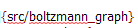
\includegraphics[height=0.2\textheight]{src/boltzmann_graph}
	\caption[Representation of a small Boltzmann machine]{Representation of a small Boltzmann machine\footnotemark}
    % https://upload.wikimedia.org/wikipedia/commons/thumb/7/7a/Boltzmannexamplev1.png/330px-Boltzmannexamplev1.png
	\label{fig:boltzmann-graph}
\end{figure}
\footnotetext{Image: Sunny vd, \url{https://commons.wikimedia.org/wiki/File:Boltzmannexamplev1.png}}

\noindent
In \cref{fig:boltzmann-graph} we can see the structure of a small BM. It consists of two layers of units which are called the visible and hidden layer.
All units in the BM are fully connected with symmetrical weights, which means that value of the weight from units A to B is identical to
the weight from units B to A. All units in a BM have a binary state of either one or zero, indicating if they are currently activated or not.
The weights can take any positive or negative real value.

The BM is used for unsupervised learning and has no clear output layer. The visible layer is used during training to hold the input data and
after learning the free running phase of the machine creates a binary vector of the states of the visible units which can be seen as the output.
The general idea behind the BM is to feed it with binary input vectors from the training dataset during the learning phase
in which the network learns the probability distribution of the set input units, which will enable it to reproduce patterns of visible units
that will match the learned probability distribution in its recall phase. A clearer explanation of the learning and recall phases follows in the 
later sections of this chapter.


\subsection{The learning phase}
Before we get into the learning algorithm of the BM, we need to introduce the concept of 'clamped' and 'unclamped' units.
As mentioned before, during the learning phase the visible units are set to the values of the binary input vectors from the training data.
This procedure is called 'clamping' the visible units, which means that during the positive phase of the learning
algorithm, the states of these units will not change and they will influence the computed states for the hidden units.

In \cref{fig:learning-alg} we can see the basic learning algorithm of the BM in pseudo code form.
The code in the figure is a simplified version of the algorithm from Cartas~\cite{BMImpl}.
To best explain the algorithm we are going to divide it into four logical parts.

\begin{figure}[p]
\begin{lstlisting}[escapeinside={(*}{*)}]
(*\textbf{\#Set up phase}*)
SET learning_epochs, co-occurrence_epochs, temperature T
SET weight matrix W = 0
LEARNING():
  WHILE W continues to change DO:
    (*\textbf{\#Positive phase}*)
    SET the sum co-occurrence matrix S = 0
    FOR EACH training pattern x:
      SET visible units to x and CLAMP them
      SET hidden units to random binary states
      CALL UPDATE-STATES(learning_epochs)
      CALL COLLECT-STATISTICS()
    SET (*$P^{+}_{ij} =$*) average (*$S_{ij}$*) over all training runs and patterns
    (*\textbf{\#Free-running phase (negative phase)}*)
    SET states of all units to random binary values and UNCLAMP them
    CALL UPDATE-STATES(learning_epochs)
    SET the sum co-occurrence matrix S = 0
    CALL COLLECT-STATISTICS()
    SET (*$P^{-}_{ij} = $*) average (*$S_{ij}$*) over all training runs
    (*\textbf{\#Update weights }$W_{ij}$*)
    Add (*$\Delta W_{ij} = k(P^{+}_{ij} - P^{-}_{ij})$*), where k is a small constant

UPDATE-STATES(epochs):
  FOR 1 to number of epochs:
    FOR 1 to number of unclamped units:
      randomly select an unclamped unit i
      Calculate its energy difference: (*$ \Delta E_i = \sum_j W_{ij} x_j $*)
      #Stochastically decide the resulting state
      IF random uniform (*$ U[0,1] < \frac{1}{1+ e^{- \Delta E_i / T}} $*):
        SET (*$x_i = 1$*)
      ELSE:
        SET (*$x_i = 0$*)

COLLECT-STATISTICS():
  FOR 1 to number of co-occurrence_epochs:
    FOR 1 to number of unclamped units:
      randomly select an unclamped unit i
      Calculate its energy difference: (*$ \Delta E_i = \sum_j W_{ij} x_j $*)
      #Stochastically decide the resulting state
      IF random uniform (*$ U[0,1] < \frac{1}{1+ e^{- \Delta E_i / T}} $*):
        SET (*$x_i = 1$*)
      ELSE:
        SET (*$x_i = 0$*)
  FOR EACH pair of connected units:
    SET (*$S_{ij} = S_{ij} + x_i x_j$*)
\end{lstlisting}
\caption{The learning algorithm}
% http://gorayni.blogspot.com/2014/06/boltzmann-machines.html
\label{fig:learning-alg}
\end{figure}

\begin{enumerate}
    \item \textbf{The setup phase:}\newline
        Before the learning algorithm can start, we need to set up some parameters. Firstly the weight matrix is initialized with zeros.
        The choice of zero, instead of an initialization with random values as it is often done for other neural networks, is
        necessary here since the weights need to be symmetric for all pairs of units as described in the introduction part of this chapter.
        The next thing to do is setting values for the temperature, learning and co-occurrence epochs. 
        The learning and co-occurrence epochs parameters will be explained in the description of the following phases.\newline
        From here on the algorithm can begin. The first thing we can see in line 4 is that the whole learning procedure (the next three steps) is
        supposed to be executed until the values of the weight matrix have converged and no more changes are observed.
        From a theoretical point of view this happens when the equilibrium state has been reached.
        In our practical implementation the while loop is replaced by a for loop with an iteration counter that can be set before the learning process.
    \item \textbf{The positive phase:}\newline
        The actual learning algorithm starts with the so called positive phase. In this phase the given input patterns are learned.
        First the units of the visible layer are set to the values of the current input vector and all visible units are clamped.
        All unclamped units (in this case the units of the hidden layer) are initialized with random binary values.
        Now the actual updating of the states takes place by calling the update function as many times as the learning epochs variable has been set to.
        This is another parameter that has to be set before the start of the learning algorithm and which has to be tuned to fit the problem.\newline
        In the update function the stochastic update of the states of the unclamped units takes place. The update calculations are done
        step-by-step for randomly chosen unclamped units. This version of the update procedure is called asynchronous and we will
        compare it to another possible version called the synchronous update, where the updates do not take place in order
        but are computed all at once in \cref{subsec:updating-procedures}.\newline
        \todo{general explanation, do it earlier? does not explicitly belong inside positive phase}
        For each chosen unit at first its energy difference is calculated with the formula
        $$\Delta E_i = \sum_j W_{ij} x_j.$$
        This is similar to other networks and lets the weights $W_{ij}$ and state $x_j$ of other units $j$ influence the current unit $i$. 
        Based on the energy difference $\Delta E_i$ then the probability $p_i$ is calculated, that the state of unit $i$ is $1$ afterwards.
        $$p_i = \frac{1}{1+e^{-\Delta E_i / T}}.$$
        The probability can then be evaluated, checking a random uniform number $u$ in range $[0, 1]$ against $p_i$.
        If $u \leq p_i$, then set $x_i = 1$, otherwise set to $0$.\newline
        Having a large weight between units $i$ and $j$ would cause a higher energy difference if unit $j$ is already set to state $1$.
        This would lead to a higher probability for unit $i$ to become $1$ as well. This should enable to memorize, that both units have often be seen together
        in state $1$. A negative weight would cause the opposite effect and enables to express both units have rarely be seen together in state $1$.
        Of course a state of $0$ would also influence the sum and a missing term can increase or decrease the energy difference and thus the probability in 
        a similar manner.\newline
        Also notice, that for a very high temperature $T$, the probability $p_i$ becomes~$0.5$, so both states $0$ and $1$ will be equally likely.
        This means high temperature leads to randomly changing states. That is not good for a final state, but helpful to explore.
        \todo{explain stochastic activation formula and stuff... was that it?}
        

        This whole procedure is repeated for all given input patterns. The last step of the positive phase is the collect statistics function which will be explained in
        the 'updating the weights' segment.


    \item \textbf{The free-running phase:}\newline
        After the positive phase the negative or 'free-running' phase starts. This phase is different to the positive phase in the fact that
        now all units of both layers are treated as unclamped. This means that also the visible layers units states can now be updated.
        Since no more input patterns are given to the visible layer all units are now initialized with a random binary value and
        the network is run freely. In this phase the previously learned information, which is stored in the weights 
        is analyzed by the network and found correlations between for example two connected units often being active at the
        same time are strengthened. The process of finding a more optimal low energy state mainly occurs in this phase.\newline
        The free-running phase is also later used to produce the output patterns of the Boltzmann machine that a user will
        look at when applying the network on a real problem.

    \item \textbf{Updating the weights:}\newline
        The updating of the weights during the learning phase is done by comparing statistics of so called co-occurring units in the positive
        and in the negative phase. A co-occurrence is the case that two units $i,j$ connected by a weight $w_{ij}$ are both observed in the
        state $1$. In the pseudo code of the algorithm these co-occurrences are summed up in the vector $S_{ij}$, where the field $ij$ is increased
        by one every time the units $i,j$ have both been observed in the state $1$.
        Since we are dealing with a stochastic process here it is necessary to collect these statistics over multiple epochs and to average
        the results afterwards. This can be seen at the definitions of the $P^+_{ij}$ and $P^-_{ij}$ variables.\newline
        $P^+_{ij}$ holds the co-occurrence statistics for the positive phase and $P^-_{ij}$ holds the statistics for the negative phase.
        It is important to recognize that the collection of the statistics in the algorithm only starts after a good amount of 
        update steps have already been done for each phase. This is needed because we can only make meaningful assumptions about 
        co-occurrences after each phase had a little time to already move towards converging on a low energy state.
        The 'collect-statistics' function then repeats a number of update steps during which all co-occurrences are summed up.\newline
        The actual changing of the weights happens after each time a pair of positive and negative phases has finished.
        Here the values of $P^+_{ij}$ and $P^-_{ij}$ are compared for every connected pair of units and their weight
        is increased by a set learning factor $k$ if there where more co-occurrences observed in the positive phase over the negative phase
        or it is decreased if less co-occurrences where observed in the positive phase. This process reinforces the learned co-occurrence 
        information from the input patterns. If during the positive phase where the visible layer is clamped to a specific pattern
        two units often showed a co-occurrence that means that this information should be learned and it will therefore
        be reinforced by changing their weight correspondingly. If however in the free-running phase two units
        are co-occurring more often than in the positive phase this does not represent the learned data properly and
        the probability of this co-occurrence has to be decreased by a corresponding change of weights.\newline
        This whole process of collecting the co-occurrence statistics and then updating the weights is done for
        every iteration of the learning algorithm. It should in the end lead to a network that in its free-running
        phase will produce visible layer patterns that represent the distribution of the learned input patterns
        as closely as possible.

        \todo{Use this reference?}
        % \cite[Chapter~43]{MacKay}\todo{didn't read, just copied reference from Cartas}
\end{enumerate}

\todo{summarize the algorithm, alternating positive/negative phase...}


\subsection{The recall phase}
\label{subsec:recall}

What we will call the recall phase in this paper describes using the previously trained BM to create output patterns.
As we have already discussed the BM only consists of one visible and one hidden layer and does not have a clear output
layer like many other commonly used neural networks. Therefore the so called outputs of the machine are considered as the patterns
in the visible layer which are created when a free-running phase is started on the trained network.
There are multiple ways in which one can use this recall to produce meaningful results. The simplest one is to just let the
machine run a few epochs in a free-running phase with all units being unclamped. In this configuration the basic idea behind the
BM comes through and the different resulting patterns in the visible layer and their probability of occurrence should
resemble the probability distribution of the learned input data. For example if the network is trained with a dataset
that contains one specific pattern five times and another pattern only once the probability of the recall to produce the first
pattern should be five times as high as the probability of producing the second pattern. Due to the stochastic nature of the BM
it is of course more likely that the resulting patterns from the recall might not exactly match one of the two inputs
but only closely resembles them. This behavior of course gets more common as the size of the input data increases.
With this use case we can already see how the BM could be used to extract key features from input datasets.
The results might not reproduce one distinct input but they should with high probability create an output that strongly
features commonalities between the different inputs.

A different approach of using the recall phase is to not start a completely free-running phase but to also add some incomplete
input data to the visible layer. This can be achieved by setting the states of some visible units to fixed values and then 
clamping those units before executing the update procedure. A simple example for this is the reconstruction of images
with broken or missing pixels. A BM is first trained with a set of images and in the recall phase
is given a partial input image. Some of the visible units are initialized with the data from the partial image and clamped.
The rest of the visible layer and the whole hidden layer are left unclamped and the update procedure is started.
After running for a few epochs the resulting states of the visible layer are taken as the outputs and they should
resemble a reconstructed version of the whole image with good probability.

One last version of using the recall phase is to create an artificial output layer for the network by dividing the visible layer
into two distinct parts at the creation of the network. This has for example been done in the original paper on the BM~\cite{Ackley}. 
Here the task was to solve a simple pattern matching problem called 'the encoder problem'.
Without going into too much detail the idea was that there are input patterns of $n$ bits that match to specific output
patterns of also $n$ bits. To learn this problem the general BM has to be slightly modified.
At creation the visible layer is divided into two $n$ unit layers which will not be interconnected but only have 
connections inside themselves and to the hidden layer. The input layer so to speak communicates with the output layer
through the hidden layer. This approach could probably also be used to solve classification problems but it
is questionable if the BM would be a good choice for this since there exist a lot of other 
networks and algorithms which solve these problems more efficiently.\newline

After describing the different possible use cases for the recall procedure we will now take a short look at 
the recall algorithm. The algorithm itself is not much different from the 
procedures we have already seen in the learning section. The basic idea is to just run the update function
for a given number of epochs in a free-running phase and to then return the resulting states of the
visible layer as outputs. Depending on which of the approaches described above is being used the only
difference is to decide which visible units should be clamped and to initialize them. 
All unclamped units are initialized with random binary values and the update procedure is called 
and returns the whole visible layer as output at some point.


\subsection{Asynchronous vs. synchronous updating}
\label{subsec:updating-procedures}

One of the disadvantages of the original version of the BM is its computational efficiency.
Firstly the learning algorithm requires the production of a lot of independent random numbers which can be costly.
The main concern however is that the original algorithm is not suited very well for parallelization.
This is a very strong concern since modern hardware relies heavily on the use of parallel code execution to
achieve good performance. This is true for today's multi-core CPUs as well as for GPU computing.
If we take a closer look at the previously seen update procedure shown in \cref{fig:update-alg}
we can see in line 4 that inside the loops each update is performed on a single unit in a randomly chosen
order. This behavior is actually required to conform to the underlying theoretical proof for the BM's
algorithm. This stems from the fact that the resulting state of one unit will influence the calculations to
determine the state of the next chosen unit. This version of the update procedure is called the asynchronous version.
This approach pretty much prohibits the parallelization of the update procedure and it impacts heavily on the performance
of the BM and therefore limits the sizes of the layers if the algorithm is expected to finish in a reasonable time.

\begin{figure}[h!]
\begin{lstlisting}[escapeinside={(*}{*)}]
  FOR 1 to number of epochs:
    FOR 1 to number of unclamped units:
      randomly select an unclamped unit i
      Calculate its energy difference: (*$ \Delta E_i = \sum_j W_{ij} x_j $*)
      #Stochastically decide the resulting state
      IF random uniform (*$ U[0,1] < \frac{1}{1+ e^{- \Delta E_i / T}} $*):
        SET (*$x_i = 1$*)
      ELSE:
        SET (*$x_i = 0$*)
\end{lstlisting}
\caption{The asynchronous update algorithm}
% http://gorayni.blogspot.com/2014/06/boltzmann-machines.html
\label{fig:update-alg}
\end{figure}

To solve this performance issue a variation of the update algorithm exists which can be parallelized.
This version is called the synchronous update procedure, and was already an option for Hopfield networks~\cite[Chapter~43]{MacKay}.
Here the calculations for the state updates are
all done in one step on all unclamped units. This at least in theory introduces some inaccuracies.
It is however not clear whether these inaccuracies have a strong impact on the practical use of the
BM and the use of the synchronous update procedure provides the big advantage of
being parallelizable. In the implementation and results parts of this paper we will
compare both of these update procedures and try to give qualitative metrics to measure
the impact of using the synchronous update over the asynchronous one.



\section{Implementation}
\label{sec:impl}

Based on the Python implementation from Cartas~\cite{BMImpl}, we generalized to allow some more flexibility by parameterization. Also we replaced a lot Python \textit{for}-loops with equivalent expressions using NumPy functions, in order to speed up the execution. As a new feature the choice between synchronous and asynchronous update method is introduced.

The idea was to bring the BM to the current world of neural networks, that offers frameworks like TensorFlow\footnote{\url{https://www.tensorflow.org}} or PyTorch\footnote{\url{https://pytorch.org}}. But the BM is a stochastic neural network, uses its own energy-based minimization process and does not use activation functions or backpropagation. The BM would not utilize any of the builtin tools these frameworks offer, and thus is hard to integrate. 

Finally we tried to use TensorFlow just for its access to GPU computation, leaving the idea of a proper integration behind. The approach to replace the NumPy calls by their corresponding TensorFlow calls was not that straight forward. We achieved some progress, but the full task could not be completed within the time frame of this seminar.\newline

Our final implementation of the Boltzmann machine can be found on github\footnote{\url{https://github.com/oliver-pola/BoltzmannMachine}}. We tried to make it as generalised as possible
so that our Boltzmann python class can be used quite easily on all kinds of problems that one might use a BM for. The final code has a low number of dependencies and should be
easy to use. It is almost purely build with the use of numpy, which should be easy to install for any user.
At the creation of a Boltzmann class instance a list of free parameters can be adjusted to fit the current use case:
\begin{itemize}
    \item \textbf{Size of visible layer}: This should simply be set to the size of the input patterns that will be learned
    \item \textbf{Size of hidden layer}: A free parameter that
        has to be tuned to the problem. In our tests we could
        not find a good general recommendation for the size
        of the hidden layer in respect to the visible layer size.
        Intuitively the hidden layer should be as as large as possible to allow 
        the BM to store as much information as possible. The drawback of this is however
        a strong increase in runtime. In practice the hidden layer size should 
        probably be set close to the size of the visible layer to make good use of it and
        at the same time not cause too much of an increase in the runtime.

    \item \textbf{Size of output layer(optional)}: This is an optional
        Argument which in the general use case can just be set to zero.
        The function of an so called output layer is to allow use cases as
        for example the encoder-problem which was described in \cref{subsec:recall}, where
        the visible layer needs to be split into two parts that are not interconnected.
    \item \textbf{Annealing shedule}: This argument expects a list of tuples of the form
        \lstinline{(<temperature>, <epochs>)}. These are the values for temperature and the
        number of epochs which will be used in the learning phase of the BM.
        In the general case a single tuple should suffice here but our implementation also
        supports the so called annealing method for learning where the learning phase
        is started with a high temperature which is then slowly decreased over time.
    \item \textbf{Co-occurrance shedule}: This argument again takes a tuple of the form
        \lstinline{(<temperature>, <epochs>)}. This is the temperature and number of
        epoch which is spend in the \lstinline{COLLECT-STATISTICS} part of the
        learning algorithm. The temperature chosen here should match the learning
        temperature in most cases but the number of epochs can differ since we
        only need enough epochs to get meaningful values for the update-weights
        part of the learning algorithm.
    \item \textbf{Synchron update flag}: Lastly it can be decided if the asynchronous or
        synchronous update procedure should be used.
\end{itemize}

The final code can as mentioned before be found in our github repository along
with the code that was used to create the results in \cref{sec:results}.


%\section{Variants}
%\label{sec:variants}
%
%When we have an implementation that can do what code of others can do as well, we will try to contribute some new approaches and maybe enlarge the scope of problems a BM can be used for.
%
%
%\subsection{Time series data}
%\label{sec:variants:subsec:timeseries}
%
%So far a BM was only applied to static data.
%
%
%\subsection{Continuous data}
%\label{sec:variants:subsec:continuous}
%
%So far a BM was only applied to discrete data.


\section{Results}
\label{sec:results}

To apply the BM on a simple but not too minimalistic problem, we use the MNIST dataset\footnote{\url{http://yann.lecun.com/exdb/mnist/}}~\cite{MNIST} containing $60000$ images of handwritten digits with labels. Each image is $28 \times 28$ pixels with grayscale values. Scaling the values to $[0,1]$ would be a good example for using the pixel values as continuous state data. But so far the BM is made for binary states and we applied the midrange threshold to get $\{0, 1\}$ pixel states.


\subsection{Recall digit pixels}
\label{subsec:recall}

From all the digits we picked only the digits 3, 4 and 5 and only a few examples in total. Then we trained the BM on this subset, having one input for each pixel and no output.
The size of the hidden layer is chosen to be equal to the input layer. The hidden layer is an important feature of the BM in opposition to a Hopfield network. The chosen size should provide the BM with some learning capacity, but due to time restrictions this parameter is not further evaluated.

The chosen total amount of epochs and the temperature are based on the evaluation in \cref{subsec:meta}. The other meta-parameters are based on examples~\cite{BMImpl} and on small exploratory sample runs, but not evaluated in detail.

\begin{figure}[t!]
	\begin{center}
	a) 10 images learned
	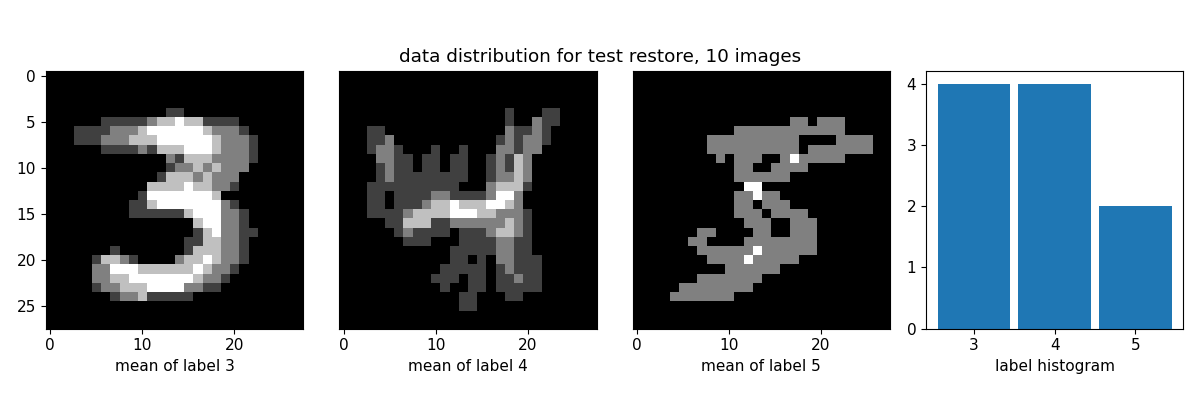
\includegraphics[trim={0.2cm 0.5cm 0cm 1.7cm},clip,width=0.79\textwidth]{src/data_distribution_10_images}
	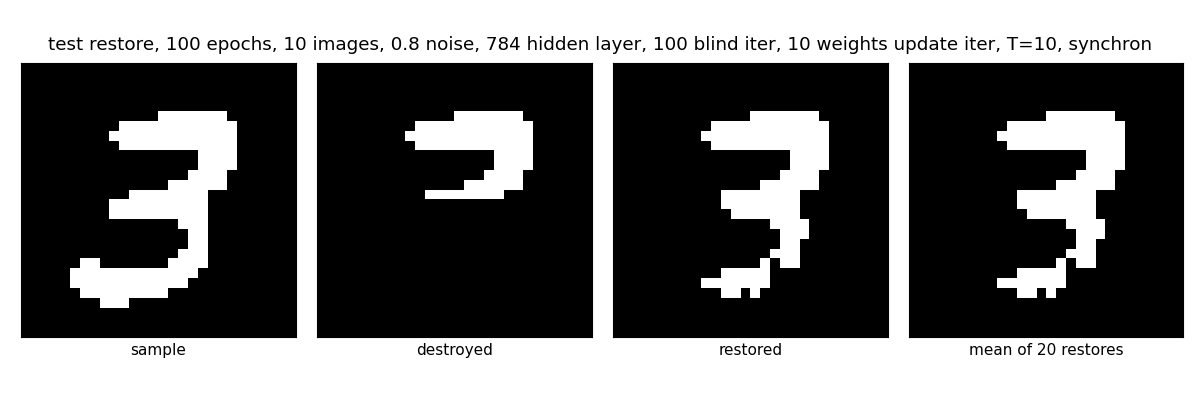
\includegraphics[trim={0cm 1.0cm 0cm 0cm},clip,width=0.8\textwidth]{src/test_restore_10_images}\\
	b) 100 images learned
	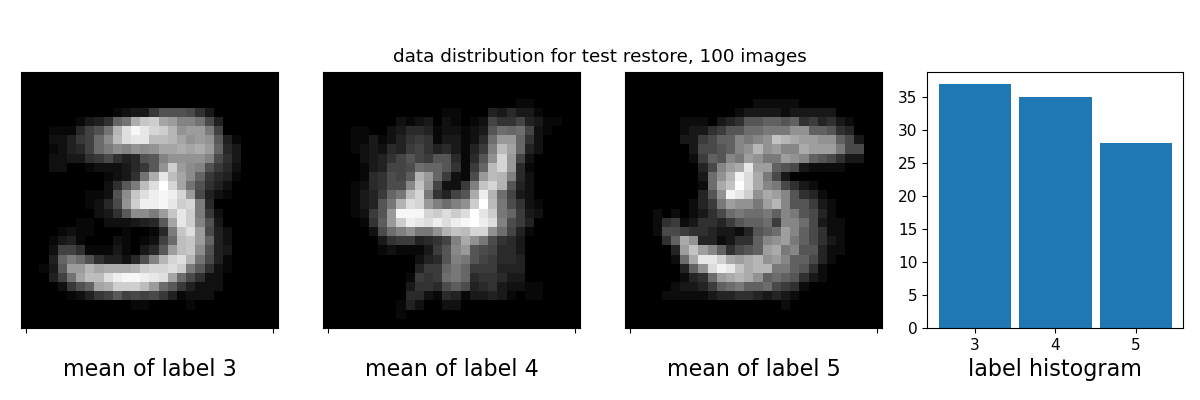
\includegraphics[trim={0.2cm 0.5cm 0cm 1.7cm},clip,width=0.79\textwidth]{src/data_distribution_100_images}
	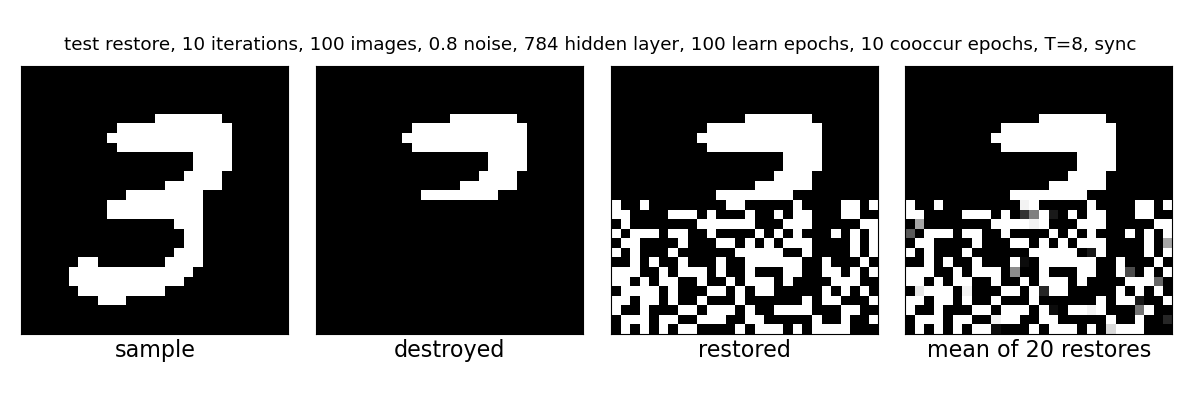
\includegraphics[trim={0cm 1.0cm 0cm 0cm},clip,width=0.8\textwidth]{src/test_restore_100_images}
	\end{center}
	\caption{Restoring MNIST digits after a) 10, b) 100 images were learned}\label{fig:test_restore}
	\footnotesize The BM did learn the sample digit 3 to restore, but also did learn other versions of the digit 3 and digits 4, 5 as well. From that sample the lower half is deleted and then restored by the BM. In a) we can see a successful restore of the pattern. The result of b) is not satisfactory.
\end{figure}

To test if the BM is able to recognize the shown patterns, we picked one of the shown digits, deleted the bottom half of it and used the BM to restore the missing pixels. We tried the recall multiple times and computed the average of the results to get an idea about the distribution. We always used the same sample and deleted the same pixels, so that the task does not vary in difficulty, knowing that the BM is unable to exploit that.

Figure~\ref{fig:test_restore} shows the distributions of the input images and the results of the recalled half pattern. 
If only 10 different images are used for training during 100 iterations, the restored digit can be identified very well, although it is not exactly the missing half.
If instead of repeating the same image many times, we show some more variations of each digit, 100 images in total, the result is not satisfying.
One reason might be if the variations differ too much, but the mean over the shown label~3 images shows, that there is not that much variation and the result should have been better.

We also can see that there is not much variation in calling recall more than once and the same output seems to be given each time. \todo{Why is that?}


\subsection{Meta-parameter evaluation}
\label{subsec:meta}

Having seen a good result from the experiment with 10 images in \cref{subsec:recall}, that same set of meta-parameters is now used as a base for further analysis on the learning phase.

\begin{figure}[b!]
	\begin{center}
	\begin{overpic}[trim={0.1cm 0cm -1.8cm 0cm},clip,width=\textwidth]{src/test_restore_quality_10_images_vary_epochs}
		\put (0,28) {a)}
	\end{overpic}
	\begin{overpic}[trim={0.1cm 0cm 0.4cm 0cm},clip,width=\textwidth]{src/test_restore_quality_10_images_vary_temperature}
		\put (0,30) {b)}
	\end{overpic}
	%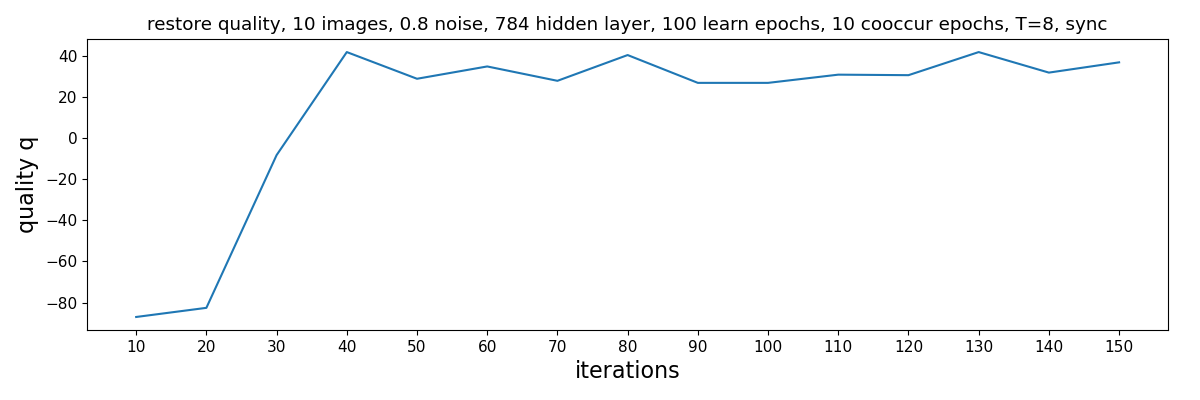
\includegraphics[trim={0cm 0cm 0cm 0cm},clip,width=\textwidth]{src/test_restore_quality_10_images_vary_epochs}
	%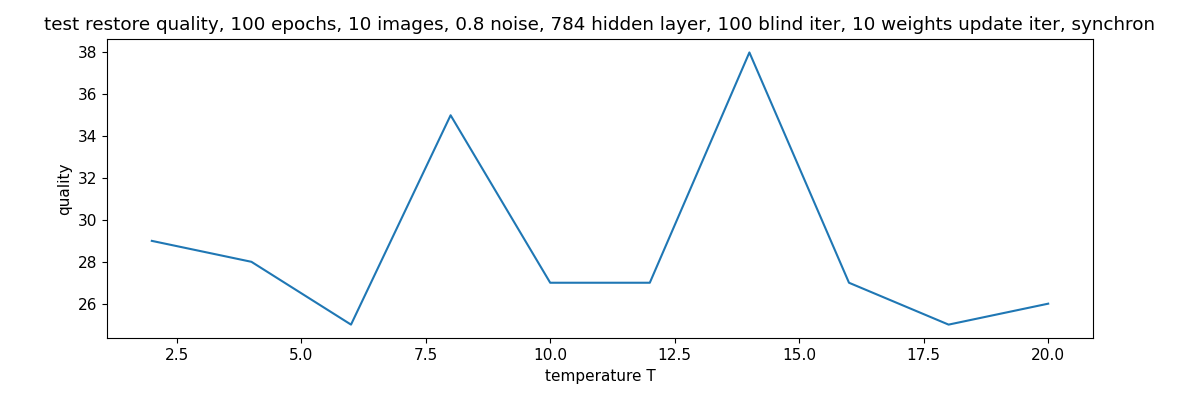
\includegraphics[trim={0.1cm 0cm 1.2cm 0cm},clip,width=\textwidth]{src/test_restore_quality_10_images_vary_temperature}
	\end{center}
	\caption{Evaluation of meta-parameters a) amount of epochs and b) temperature}\label{fig:test_vary_epoch_t}
	\footnotesize On the same experiment from \cref{subsec:recall}, the learning phase is repeated for every data point on the x-axis. After recalling the pattern, the quality is measured by $q$ and displayed on the y-axis.
\end{figure}

While all other meta-parameters are kept fixed, the same experiment is performed, but with varying total amount of epochs and temperature.
To have a scalar to measure the quality $q$, a simple approach using the pixel values $x_\text{sample}(i)$ from the original and $x_\text{restore}(i)$ from the restored pattern at the same coordinate $i$ is applied.
The left term rewards pixels set in the restored pattern where a pixel was set in the original, and the right, negative, term punishes restored pixels where no original pixel was set:
$$q = \sum_{i : x_\text{sample}(i) = 1} \frac1{20}\sum_{\text{20 recalls}}x_\text{restore}(i) - \sum_{i : x_\text{sample}(i) = 0} \frac1{20}\sum_{\text{20 recalls}}x_\text{restore}(i)$$
The results in \cref{fig:test_vary_epoch_t} a) show that, at least for 10 images only, the results will not get better extending the number of epochs.

About temperature $T$ is known that at $T=0$ the BM is no longer stochastic, but deterministic. The higher $T$, the more unknown states are tested, instead of staying at the known minimum so far. A too high $T$ though will just cause a lot of noise. From this, a quality maximum is expected for some mid-range $T$.

The course seen in \cref{fig:test_vary_epoch_t} b) is not expected and without explanation.
To gain information out of this, an average over many runs of this experiment would be needed, but was not conducted due to time restrictions.
Peaks at very low $T$ are considered as lucky initial randomness in this instance, whereas higher $T$ is considered to be of more random nature. The peak at $T=8$ seemed to be most stable and was chosen to be the base value for our experiment.

As the synchronous update was implemented to benefit from easier parallelization, we focused to tune the meta-parameters for this version. \cref{fig:test_vary_epoch_t} shows that the behavior is different.
For the chosen set of parameters the synchronous update is more stable and does not degrade when continuing learning for more epochs.
Another set of parameters might be the sweet spot for the asynchronous update to reach this stability.


\section{Discussion}
\label{sec:discuss}

The discussion of the results may be included in the results chapter and not be worth a separate one. % TODO


\section{Limitations}
\label{sec:limits}

Since this is an implementation topic, the main limitations derive from our implementation and may be discussed in that chapter. So this might not result in a chapter on it's own. % TODO


\section{Future Work}
\label{sec:future}

(May be covered in the final version of this paper)\\

\noindent
The BM as it was defined and used in this paper is only applicable to static discrete data. As already mentioned when using the MNIST images, we therefor had to adjust or pixel values in range $[0,255]\cap\mathbb{N}$ to be binary $0$ or $1$ via threshold. It would be nice to directly use values in continuous range $[0,1]$ instead. Where we currently set the new state to $1$ with probability $p$, this could be achieved by directly setting the new state to $p$. The other parts of the algorithm then need to be adapted as well.

As the BM is a recurrent neural network, a proper application seems to be time series data. This also seems to be where the Restricted BM is applied, that we have chosen not to cover in this paper. But it might to be possible to adapt the general BM to this task as well.


\section{Conclusion}
\label{sec:concl}

We will conclude with our interpretation of the results and will point out where future work would be beneficial.


%%%%%%%%%%%%%%%%%%%%%%%%%%%%%%%%%%%%%%
% hier werden - zum Ende des Textes - die bibliographischen Referenzen
% eingebunden
%
% Insbesondere stehen die eigentlichen Informationen in der Datei
% ``bib.bib''
%
\newpage
\bibliographystyle{plain}
\addcontentsline{toc}{section}{Bibliography}% Add to the TOC
\bibliography{bib}

\end{document}


